\section{System Implementation}
\begin{figure}[h]
\centering
  % Requires \usepackage{graphicx}
  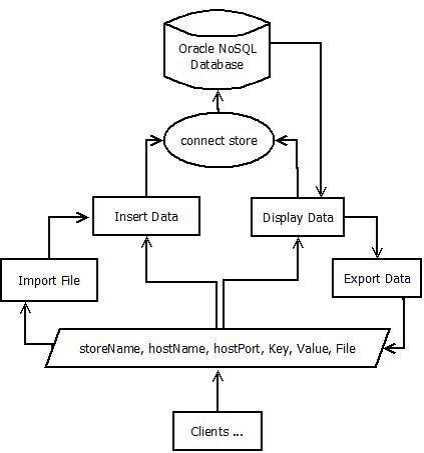
\includegraphics[width=12cm,height=10cm]{Fig21.jpg}\\
  \caption{System Architecture}
  \label{System Architecture}
\end{figure}
\begin{itemize}
  \item \textbf{Part1}
\end{itemize}
The system is a web application which fits into the application logic layer of three tier Architecture. System provides the ease to access key-value paired Oracle NoSQL database. System is a web interface through which the user can connect to the database and perform required operations. Position of the System in Three Tier Architecture is shown in figure
\\
\hspace*{0.7in} System's interface provides with various functionalities on database which includes CRUD operations and Import Export. The System follows disconnected architecture. in disconnected architecture the system is not synchronized with another system. System works in three stages i.e. connect to data store, perform operations and disconnect from data store. For performing every new operation the system needs to follow above three steps. System follows disconnected architecture then too system maintains session, in sessions Store Name, Host Name and Host Port are stored. Because foe every new operation user should not have to enter again those parameters.
\\
\hspace*{0.7in} The system interface is kept simple, so that any user having basic knowledge of key value based NoSQL database can use the system. The System is developed as a User Interface for Oracle NoSQL Database. System uses KVLITE which is a Single Node Data Store by Oracle NoSQL. The System uses kvclient.jar file which has all the necessary library files for using KVLITE or KVSTORE.
\\
Following operations can be performed using the Developed System:\\

\begin{enumerate}
  \item Connect to Store : \\
\hspace*{0.7in} This function connects the client to Data Store on Remote Server. this functions takes three parameters namely Store Name, Host Name i.e. host address on which the data store is installed and Host Port i.e. on which the Data Store's service is started. When the system connects to data store a new session is created and this session is maintained until the user completes specific operation or logs out from system.

  \item Insert Data : \\
\hspace*{0.7in} This function is used to insert Single or Multiple Key Value pairs in the Data Store. The function comes in two forms i.e. Single and Multiple Key Value Pair Insert. For Single Key Value Pair insert system requires three parameters, namely Major Key Component, Minor Key Component and Key Value. For Multi Key Value Pair Insertion the system first asks for Major Key Component and Minor Key Component Count, followed by that the user has to enter Minor Key Components and Key Values.

  \item Display Data : \\
\hspace*{0.7in} This function gets the data from the store and displays to user. Functions come in two forms i.e. Single and Multiple Key Value pair display. For Single Key Value display system takes Major Key and Minor Key Component and parameters. And for Multi Key Value pair display System takes only Major Key Value Component.

  \item Update Data : \\
\hspace*{0.7in} This function is used to update the existing Key Value pairs. This function also comes in two forms Single and Multiple Key Value Pairs Update. For Single Key Value Pairs update user has to enter Major Key Component, Minor Key Component and Key Value. And for Multi Key Value pair update user has to enter one Common Major Key Component and its Minor Key Components along with Key Values.

  \item Delete Data : \\
\hspace*{0.7in} Delete functions is used to delete existing Key value Pairs. The function has two forms. The first form is Single Key Value Pair delete where user has to enter Major and Minor Key Component. And for Multiple Key Value pair delete user has to enter only Major Key Component.

  \item Import Data : \\
\hspace*{0.7in} The function provides Import functionality. Here the data can be imported from a Comma Separated value file into the database. Here firstly user has to upload a file to server which is to be imported into the data store. After the file is been uploaded the system ask user to mention Major Key Component and Minor Key Component for that file along with the Minor Key Part. Here the Minor Key Component is a composite form of Minor Key Component specified by the user and a field from CSV file. These two parts makes a new Minor Key which is used to identify the Key Value Pair uniquely. This approach is used so that the Relational Database can be mapped with NoSQL Database.

  \item Export Data : \\
\hspace*{0.7in} Here the data from database is directly exported into the CSV (Comma Separated Value) file. The data which is to be exported is firstly fetched from database and if user wish to export that data into file then that data is exported into the CSV file. This function is only available for multiple Key Value pairs Export.
\end{enumerate}

\begin{itemize}
  \item \textbf{Part2}
\end{itemize}
\hspace*{0.7in} The Part 2 of project consists of Creating Web Services to access the NoSQL database. Web services are developed so that the any client independent of any platform can access the database. Here in our application RESTful webservices are developed. RESTful, because this are stateless and lightweight. This web services are meant to access from mobile devices. \\
\hspace*{0.7in}	In our case to demonstrate the use application of big data, Sensor generated data is stored and is access from the KVStore. This sensor data is gathered from the Bio Metrics Thumb machine use for daily attendance record. \\
\hspace*{0.7in}	Here two web services are created:
\begin{enumerate}
    \item To get the daily attendance of user : \\
\hspace*{0.7in} Here User gets the date wise attendance report. The user has to enter his/her user id In/Out log and Date and Log in or Log out Time is displayed to the user.

    \item To get the monthly attendance of the user : \\
\hspace*{0.7in} Here user gets the month wise attendance report. The user has to enter his/her user id and the respective month and year and the monthly attendance is displayed by calculating it from working days.
\end{enumerate}

\begin{itemize}
  \item \textbf{Part3}
\end{itemize}
\hspace*{0.7in} Android application is been developed through which the user gets his/her attendance report. The above explained web services are been consumed using this application.


\section{Mathematical Modeling and algorithm}
This mathematical model represents the proposed system described in the previous section.
$\bigodot S=\{\Sigma,q0,\delta,F,Q\} $ \\
Where \\
$\Sigma = \{ $ storeName, hostName, hostPort, majorKeyComponent, minorKeyComponent,  keyValue $\}$ \\
q0 = {Connect to Store} \\
$\delta$ = {f1 , f2 , f3 , f4 , f5 , f6 , f7} \\
f1= connectStore \\
f2 = insertSingleData \\
f3 = insertMultiData \\
f4 = displaySingleData \\
f5 = displayMultiData \\
f6= updateSingleRecord \\
f7= deleteSingleRecord \\
f8= deleteMultiRecord \\
f6 = importCSV \\
f7 = exportCSV \\
Q = {Connect to Store, Perform Operation, Disconnect from Store}
(All functions from f1 to f6 are already explained in previous section)


\subsection{Applications}
\begin{itemize}
  \item For managing key value paired oracle nosql database.
  \item For importing and exporting data from Oracle NoSQL Database.
  \item For attendance check to employees in organizations.
  \item The GUI based application can be used anywhere, where Oracle NoSQL databse comes into focus.
\end{itemize}

\subsection{Advantages and Disvantages}
\begin{itemize}
  \item Reduces efforts and time of user for managing Oracle NoSQL Database.
  \item Direct Import Export Functionality.
  \item REST Ful web services whose functionalities can be extended on any platform for any use.
\end{itemize}
